\setchapterpreamble[u]{\margintoc}

\chapter{Droplet Generation in Corrugated Ligaments}
\labch{breakup}

% Rearrangement of liquid volumes in ligaments
Ligaments constitute the penultimate stage in the complex sequence 
of capillary-driven topological changes that are 
typical of liquid fragmentation processes, 
finally resulting in the generation of polydisperse collections of drops. 
In the context of the present body of work, we shall 
only concern ourselves with the dynamics of Newtonian ligaments, 
which are well described by the Navier-Stokes equations 
at the incompressible and isothermal limits. 
The rearrangement of the liquid volumes that constitute
the ligaments play a key role in determining the size 
of the droplets that emerge immediately after the disintegration
of the thread-like structure (Fig. \ref{lig_stretch} ).  

\begin{marginfigure}[3cm]
\centering
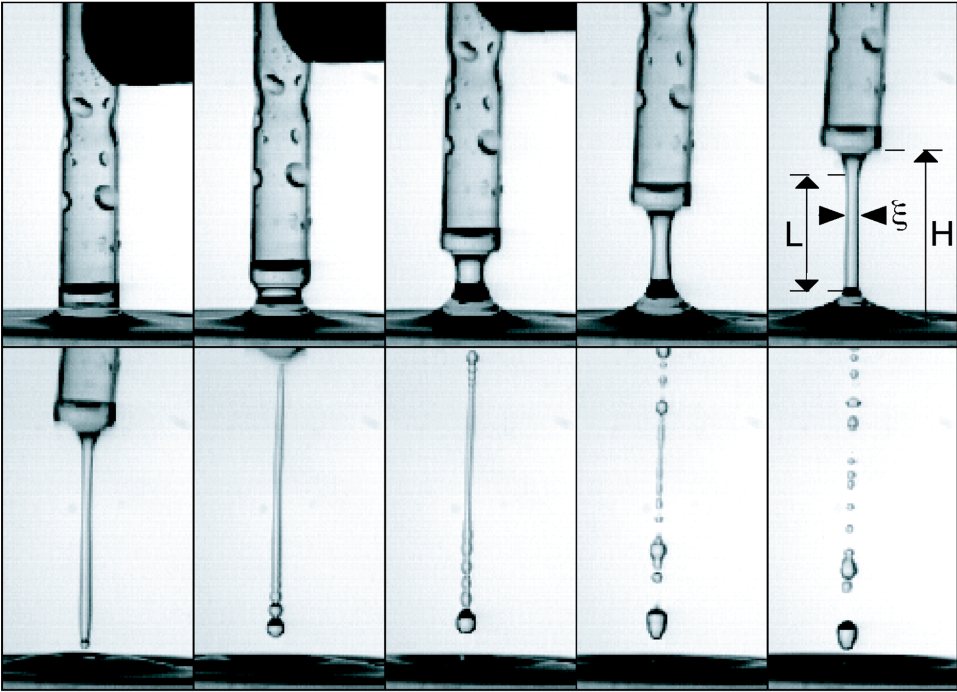
\includegraphics{plots/ligament_breakup/lig_mar_vill_pof04.png}
\caption{Fragmentation of stretched liquid (Newtonian) ligaments formed 
	immediately after retraction of a capillary tube. 
	Image reproduced from Marmottant \& Villermaux \cite{vill_3}.
       	The complex rearrangement of the liquid volumes 
	inside the ligament plays a key role in its subsequent 
	disintegration into droplet of various sizes. 
	}
\label{lig_stretch}
\end{marginfigure}

The dynamics of these rearrangements prior to breakup are 
governed by non-linear interactions between several 
physical mechanisms such as the growth and propagation of capillary 
waves along the ligament surface, remnants of the internal flow, 
stretching induced either by the surrounding gas flow or by 
acceleration of the liquid into the surrounding medium itself,
not to mention the dissipative effects of viscosity.  
Although we present a convoluted picture of ligament dynamics prior
to breakup, it is ultimately the capillary force that drives the 
eventual topology change from the thread-like structure to that of the drop. 
The primary role of the both the inertial and viscous forces is to oppose 
or dampen the destabilizing effects of the capillarity induced deformations.   
An additional mechanism to consider is the merger or coalescence of the 
newly created droplets (post-breakup) along the axis of the former ligament
structure, or with droplets originating from other sources in the near vicinity. 
The generation of drops whose diameters are significantly larger than the 
width of original ligament are predominantly driven by the aforementioned coalescences.  
Therefore, considering the combined effects of the above mechanisms, we expect a significant
departure of the resulting drop size distribution from that predicted by the  
classical analysis of the Rayleigh-Plateau instability \cite{rayleigh1879a,rayleigh1879b}. 


% Corrugation-coalescence model
\section{Coalescence Cascade}

Linear theory based on the Rayleigh breakup of infinitely
long liquid cylinders in a quiescent medium predicts the disintegration
of the thread along regular intervals, the length of which is governed
by the fastest growing spatial frequency. 
The drops generated according to this model would be uniform in
size, in sharp contrast to the significant variances in the size distributions
observed in reality.  
Even in the simpler case of decaying liquid jets, 
non-linearities near the breakup zone kick into effect beyond
the initial exponential growth phase predicted by linear theory, 
eventually resulting in the jet breaking up into 
``main'' drops and significantly smaller ``satellite'' droplets 
\sidenote{Refer to the high quality photographs in 
the work of Rutland and Jameson \cite{rutland1971non}, where they demonstrate 
the formation of ``satellite'' droplets that manifest due to the non-linear effects
driving the jet breakup.}. 
Thus, simply taking into account the non-linear effects driving the breakup would
lead to a bimodal distribution of droplet size, but this explanation 
still fails to account for the broad distribution of sizes observed in 
the outcomes of the majority of natural \cite{nature} and industrial \cite{industrial} processes. 


As we have seen in the previous chapter, there are several hypotheses 
in existing literature \sidecite{vill_1} 
that attempt to model the underlying physical mechanisms 
that are responsible for the selection of droplet size. 
A model first proposed by Villermaux and coworkers \sidecite{vill_2,vill_4}
asserts that the variance in the droplet sizes is strongly 
correlated to the initially corrugated shape of the 
ligament, from which the drops originate. 
In this model, the corrugated ligament is represented as a collection 
of `blobs' (see Fig. \ref{blobs}), with the continuous interaction between 
such blobs throughout the destabilization phase accounting for the 
rearrangement and concomitant aggregation of the liquid volumes prior to breakup. 
\marginnote{
The corrugation-coalescence mechanisn has been 
popularized in several studies such as \cite{vill_3,vill_1,vill_5,vill_6,vill_7},
and more recently in \cite{bonn,mckinley}.
}
The key parameter concerning the predictions of this model 
is $n$, which characterizes the corrugations in the initial 
geometrical shape of the ligament, defined as  

\begin{align}
	n \equiv \frac{1}{\left(\langle d^{2} \rangle - \langle d \rangle^{2} \right) / \langle d \rangle^{2}} \, ,  
\end{align}

\begin{marginfigure}
\centering
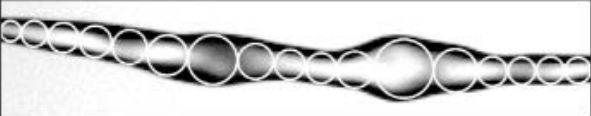
\includegraphics{plots/ligament_breakup/lig_protoblobs.png}
\caption{Representation of the liquid volumes in an isolated ligament as `blobs'
	of sizes $d$ matching the corresponding the local thicknesses, 
	just before the destabilization into droplets. 
	Image reproduced from Villermaux \cite{vill_1}.
	}
\label{blobs}
\end{marginfigure}


where the quantities in the brackets $\langle \quad \rangle$ represent the mean
and the diameters $d_i$ correspond to that of the blobs as shown in Fig. \ref{blobs}.
These studies essentially demonstrate that the degree of polydispersity 
in the drop sizes can be simply explained by examining the 
degree of ``smoothness'' in the initial geometry of the ligaments, 
with the standard deviation or distribution width of the size of the 
emerging drops scaling as $1 / \sqrt{n}$. 
As a corollary to this prediction, a broader distribution of drop sizes arise out
of the disintegration of strongly corrugated (rough) ligaments, whereas smoother 
ligaments with uniform thickness lead to a narrower (monodisperse) distributions. 


\begin{marginfigure}
\centering
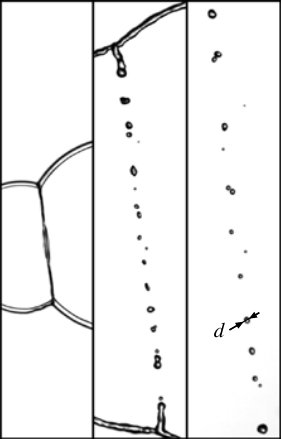
\includegraphics{plots/ligament_breakup/lig_sheet_hole.png}
\caption{Successive stages in the breakup of a ligament into drops. 
	The system shown here is that of a perforated liquid sheet, 
	where the growth of such perforations due to capillary retraction 
	of the liquid rims lead to the formation of networks of connected ligaments. 
	Image reproduced from Lhuissier and Villermaux \cite{sheet_hole}.
	}
\label{lig_network}
\end{marginfigure}


% Difficulties associated 
Over the last two decades, a handful of studies have been conducted 
with the aim of carrying out detailed observations surrounding 
the aforementioned ``coalescence cascade'', whereby the drops 
constitutive of the ligament tend to coalesce and form larger drops
as and when they detach from the initial thread-like structure.
Most notable amongst those studies is the one by Marmottant and Villermaux \cite{vill_3},
wherein they illustrate the successive stages of the disintegration of 
liquid ligaments formed when capillary tubes are rapidly retracted from 
the surface of a liquid pool (refer to Fig. \ref{lig_stretch}). 
Another set of observations were presented by Lhuissier and Villermaux \cite{sheet_hole},
where the disintegration phase sets in starting from a transient configuration
of the ligaments arranged in a spider-web like network (Fig. \ref{lig_network}).  
A more recent experiment is that of Keshavarz et al. \cite{mckinley},
which is inspired by the capillary tube retractions of \cite{vill_3} 
but directed towards the behaviour of non-Newtonian fluids.
The fundamental limitation that is common to experiments cited above 
is the inability to precisely control the initial conditions.
In other words, generating ligaments conforming `\textit{exactly}'
to a specified geometrical shape is practically (almost) impossible 
due to the inherent difficulties associated with the control of free-surface flows.  
In the absence of such precise control and reproducibility of the initial 
ligament corrugations, one has to resort to a posteriori correlations between 
the width of the final drop size distributions and qualitative descriptions 
of the initial surface profiles.
A central theme of the current chapter is concerning the design and conception
of `numerical' experiments that lend themselves to accurate and repeatable 
specifications of the initial conditions of the ligaments in question.  
An additional advantage offered by our high-fidelity numerical approach 
is the access to a much wider range (compared to physical experiments) within the 
space of all control parameters that influence the dispersion in the drop size distributions, 
not to mention the higher levels of temporal resolution on offer 
that enable better tracking of the non-linear dynamics near pinch-off
\sidenote{The characteristic time-scale of the flow near the 
vicinity of the breakup is given by $ t_{\sigma} \sim \left(\rho r^3 / \sigma \right)^{1/2} $, thus
leading to faster flows and contraction of the time-scales as the local thickness ($r$) 
decreases to zero. In our numerical methods, we can adaptively select the time
interval over which the integration of the governing equations are carried out, to 
accommodate such non-linearly accelerating flows.}. 
The combination of these two features enables us to quantitatively map the 
influence that the degree of smoothness of the initial ligament has on the ensuing 
liquid rearrangements, as well as the coalescence dynamics following the ligament. 


\section{Breakup Regimes}

\blindtext

\blindtext


\blindtext


% Brief review, eggers , Keller-Miksis and Viscous regimes


%---------------------------------------------------------------
\section{Numerical Setup}
Our numerical experiments entail direct numerical simulations of the two-phase
Navier-Stokes equations, employing the one-fluid model which  
solves only a single set of governing equations throughout the whole domain,
where the domains are composed of regions of variable density and viscosity. 
In order to reproduce the free-surface dynamics, a Volume-of-Fluid 
(VOF) approach is used to capture the interface, the explicit location 
of which marks the separation between the two fluids.


\begin{marginfigure}
\centering
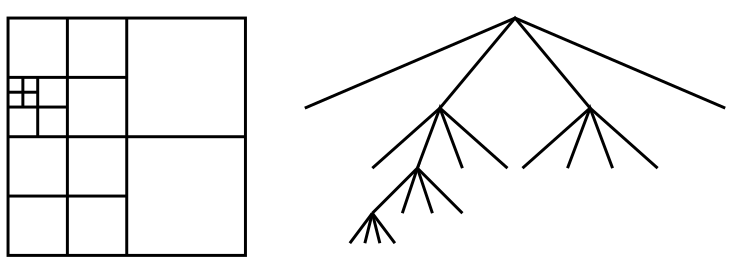
\includegraphics{plots/ligament_breakup/octree.png}
\caption{A schematic of the octree grid used in Basilisk, and its
	corresponding logical structure (quadtree in 2D).
	Image reproduced from Agbaglah et al. \cite{agbag}.
	}
\label{octree}
\end{marginfigure}


A more detailed evaluation of the comparitive advantages of different  
interfacial tracking approaches (e.g. VOF, level set, phase field etc) 
can be found in the comprehensive review by Scardovelli and Zaleski 
\cite{zaleskiannual}, or in a more recent exposition by  
Mirjalili et al. \cite{mirjalili2017interface} on the same topic.
The immiscible nature of the flows under consideration translates to the 
absence of mass tranfer across the interface, thereby rendering the 
velocity field continuous across the interface at the incompressible limit. 
The study is primarily focused on isothermal air-water systems, with 
the material properties corresponding to that at 20 degrees Celcius. 

\paragraph{Numerical Platform : Basilisk}

\begin{marginfigure}
\centering
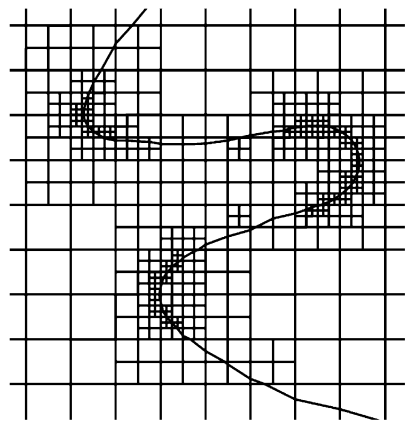
\includegraphics{plots/ligament_breakup/multi_scale.png}
\caption{ A demonstration of multiscale capabilties
of Basilisk, wherein the mesh dynamically adapts in order
to resolve the smaller scale features of the interface. 
Image reproduced from Agbaglah et al. \cite{agbag}.
}
\label{amr}
\end{marginfigure}


We solve our set of governing equations using the open-source toolbox 
Basilisk \cite{basilisk}, which couples finite-volume discretization 
on octree meshes (Fig. \ref{octree}) to solve the two-phase 
Navier-Stokes equations with surface tension.
The use of adaptive mesh refinement (AMR) in conjunction with the octree structure
allows an extremely efficient (compared to uniform grids) utilization of 
computational resources especially when dealing with the multiscale nature (see Fig. \ref{amr}) 
of surface tension dominated flows, where the bulk of the computational power
is diverted towards resolving regions in close proximity to the interface location. 
The solver utilizes a robust and accurate implementation 
of the CSF \cite{csf} (Continuum Surface Force) surface tension model 
that governs the volumetric distribution of the capillary forces on the dynamically 
refined grid (refer to \cite{popinet2009accurate} for more details). 
The numerical methods used in Basilisk have been extensively validated
through studies conducted on a variety of free-surface flows, 
recent examples being on the topic of air entrainement through wave breaking
\cite{basilisk_1, basilisk_3}, jets created due to bursting bubbles \cite{basilisk_2, basilisk_5}
modeling of viscoelastic droplet splashes \cite{basilisk_4} and many more.


\subsection*{Computational Schematic}

As discussed in the previous sections, the 
dynamics of the liquid volume rearrangements 
within the ligaments are quite involved 
due to the non-trivial interactions between
the inertial, viscous and capillary effects 
at different length and time scales that span
over several orders of magnitude.
In order to isolate the direct influence of 
initial geometrical shape of the ligament on 
the subsequent dynamics, we have decided to 
exclude the inertial forces \sidenote{
We use inertial forces as an umbrella term
to describe all the forces that might contribute to
the ``stretching'' of the ligament, 
thus opposing the capillary deformations.
These primarily include the remnant flow within
the ligament bulk, the aerodynamic shear at the interface
and the acceleration of the ligament itself into 
the surrounding gas medium. 
}
with respect to the initial conditions. 
Therefore, we opt for a very particular type of setup,
with infinitely long ligaments having zero initial kinetic energy, 
and spatial periodicity in the geometrical shape along the axis. 
We carry out the simulations in an axisymmetric framework, 
therefore excluding any azimuthal variations
in the initial shape as a consequence of this simplification. 
Fig. \ref{schematic} illustrates the a 2D schematic of the
computational setup, where the domain is a square of side $L$. 
The bottom side of the box acts as the axis of symmetry for 
the corrugated ligament (detailed view in the inset of Fig. \ref{schematic}), 
which has an unperturbed (mean) radius $R$. 
Due to the periodicity of the ligaments in the axial direction, 
we impose periodic boundary conditions for the primary variables 
on the left and right faces of the domain.
Symmetry conditions are imposed on the bottom side, 
with impenetrable free-slip conditions applied on the top side. 


\begin{figure}
\centering
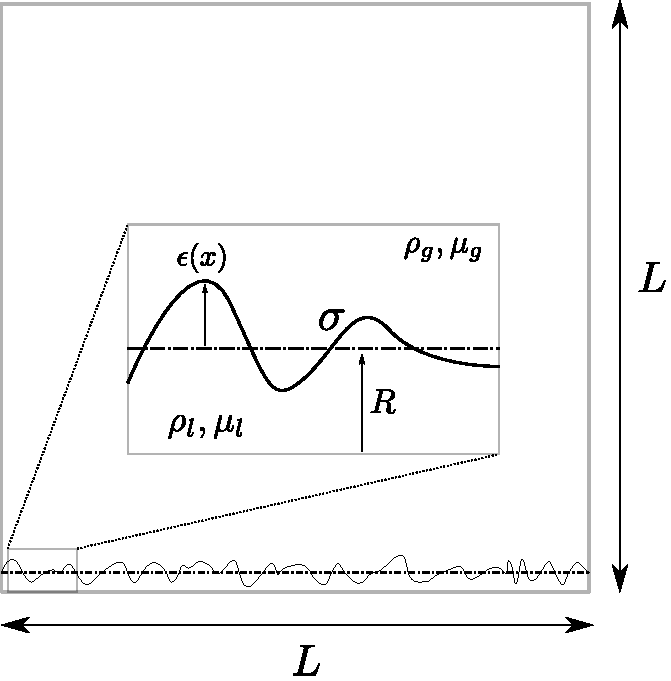
\includegraphics{plots/ligament_breakup/schematic.pdf}
\caption{ A 2D schematic of the computational domain.
An infinitely long and axisymmetric corrugated ligament
of mean radius $R$ is placed in a square box of side $L$.
The bottom side of the box acts as the axis of symmetry 
for the ligament, with spatial periodicity along the horizontal 
direction. Inset : A close up view of the corrugated profile
of the ligament, where the local radius is defined as 
the sum of the unperturbed (mean) radius $R$ and the local 
perturbation $\epsilon(x)$. The material properties of the 
liquid and gas phases are denoted with the subscripts $l$ and $g$
respectively, which in our case corresponds to an air-water system
with the surface tension coefficient $\sigma$. 
}
\label{schematic}
\end{figure}

\subsection*{Random Surface Generation}

A key ingredient of this investigation on the impact 
of corrugations is the ability to precisely
control the quantitative aspects of the initial 
corrugated surface profile of the ligament. 
Towards that objective, we construct a surface 
using the superposition of random overlapping waves, 
corresponding to an overall spatial period $L$ of the resulting profile. 
The aspect of ``randomness'' is achieved by  
using a state of the art white noise generation algorithm,
introduced in the seminal work of Matsumoto and Nishimura \sidecite{rng}.
A robust and open source implementation of the aforementioned algorithm 
is available in the GNU Scientific Library toolkit \cite{gnusl},
and thus readily incorporated into our numerical platform Basilisk.   

\begin{figure}
\centering
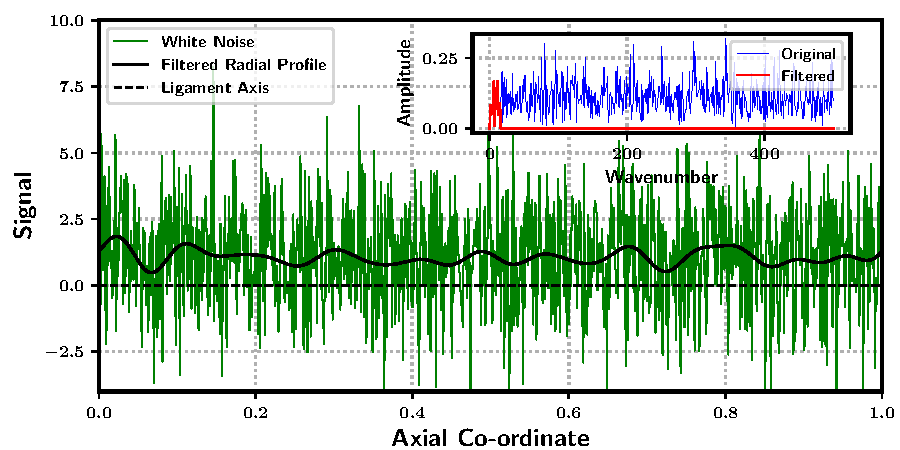
\includegraphics{plots/ligament_breakup/profile.pdf}
	\caption{ Radial profile of the noisy and the subsequently 
	low-pass filtered surface of the ligament, corresponding to 
	one spatial period along its axis. 
	Inset : Spectral densities of the initial noisy signal
        and the corresponding filtered signal. Only a handful
	of small wavenumbers are chosen to create the surface. 
}
\label{surface}
\end{figure}

The discretization of the radial profile $R(x)$ is denoted as $R_i$, 
which can be expressed as the sum of the mean radius 
(unperturbed) and some random perturbation such that    

\begin{align}
	R_i = R + \lambda_i \quad , \quad \lambda_i \sim \mathcal{N}(0,\epsilon_{0}^2) \quad , 
\end{align}

where $i$ represents the discretization of the continuous profile 
along the axis of symmetry, and $\lambda_i$ corresponds to random numbers
generated by our white noise algorithm  
\sidenote{ As one can infer from the inset of Fig. \ref{surface},
the creation of our corrugated profiles are based on the popular 
model in information theory termed as white Gaussian noise, where 
white refers to the flat spectrum in frequency space, and Gaussian 
due to the normal distribution in physical space. }, with the numbers normally 
distributed with zero mean and $\epsilon_{0}^{2}$ as variance .
The exact sequence of numbers $\lambda_i$ is uniquely determined 
by the value of the seed given as input to the white noise generator.
This ensures that there are no unforeseen correlations between the shapes of any two
ligament surfaces, even though some long range correlations are introduced
within the individual ligaments themselves due to the filtering process. 
The initial noisy surface generated by the white noise algorithm
contains extremely sharp edges corresponding to infinite values of 
interfacial curvature (see Fig. \ref{surface}), which are present due
to the inclusion of perturbations corresponding to large wavenumbers. 
\marginnote{
It is interesting to note that we can independently control 
the dispersion (standard deviation) in the final ligament profile  
via two means, first is the variance of the initial noise ($\epsilon_0$) 
and second is the threshold used for the low-pass filter. 
}
In order to avoid the ``smoothening'' of these edges by our numerical method,   
we remove these high frequency modes \textit{a priori} in a controllable fashion. 
As demonstrated in Fig. \ref{surface}, the noisy surface is treated by a low-pass filter 
in order to obtain the final description of the ligament's radial profile. 


\subsection*{Adimensional Groups}

The initial conditions of the computational setup can be 
characterized by Weber and Ohnesorge numbers, as defined below   

\begin{align}
	We = 0 \quad , \quad Oh = \mu / \sqrt{\rho \sigma R} . 
\end{align}

The Weber number is zero due to the ligaments initially being at rest, 
but during the rapid destabilization phase a part of the surface 
potential is instantly transformed into kinetic energy of the liquid.  
The Ohnesorge number is simply the square-root of the ratio  
of the viscous length scale ($l_\mu$) \sidenote{
The viscous length is defined as $l_{\mu} = \mu^2 / \rho \sigma $.
It is intrinsic to the system of the liquid and its free-surface, 
therefore is not influenced by initial conditions 
or any global parameters specific to the problem.
} 
to the characteristic length scale of the problem ($R$).
The geometrical shape of the ligament can 
be characterized by the combination of a measure of the initial
corrugation amplitude ($\varepsilon$),
cut-off wavenumber ($K$) and the aspect ratio ($\Lambda$), defined as   

\begin{align}
 \varepsilon = \epsilon_0 / R \quad , \quad K = n_c \cdot \left(2\pi W/ L \right) \quad
	, \quad \Lambda = L / W , 
\end{align}

where $W = 2R$ denotes the mean width of the ligament, with only
the $n_c$ smallest (discrete) wavenumbers passing through the low-pass filter .
\marginnote{
The volume of the corrugated ligament per unit spatial period 
is controlled by the aspect ratio, thus indirectly setting the 
upper limit to the size of the largest drop that could thoeretically
form if all the volume of the ligament were to congregate into a single shape.
}
As in the case with most surface tension dominated flows, 
the capillary time scale ($t_\sigma = (\rho R^3 / \sigma)^{1/2}$) is the most 
natural choice of time interval by which we can rescale our physical time.
Thus, our non-dimensional time is given by 

\begin{align}
	T = t \cdot \left(\rho R^3 / \sigma \right)^{-1/2} . 
\end{align}


\subsubsection*{Active Wavenumbers}

As a consequence of the discrete nature of space in
the context of numerical simulations, we can inject energy
only into certain spatial frequencies \sidenote{
In our particular case, only the modes corresponding to 
the the longest $n_c$ wavelengths ($L$, $L/2$, $L/3$ ... $L/n_c$) 
are left with any excitation once the initial noisy profile is 
passed through the low-pass filter.}. 
The general and important result that a liquid cylinder is unstable 
only to perturbations of wavelength larger than $\pi$ times the diameter
is was first demonstrated in the original work of Plateau \cite{plateau1849}.
The subsequent evolution of these low frequency modes  
is determined by the dynamical response of the system in question, 
subject to the underlying governing equations. 
In the context of inviscid flows, the dispersion relation
resulting from linear stability analysis of the potential flow
inside a liquid cylinder subject to sinusoidal perturbations is given by

\begin{align}
\omega = \frac{\omega_0 I_1(x)}{I_0(x)} \left(1 - x^2 \right) , 
\label{rayleigh_plateau}
\end{align}
 
\marginnote{ $I_0$ and $I_1$ are modified Bessel's functions of the 
first kind, corresponding to order $0$ and $1$ respectively. 
Detailed derivations of \eqref{rayleigh_plateau} and \eqref{weber_chandra}
can be found in the comprehensive review by Eggers \cite{eggers1997nonlinear}.
}

where $\omega_0 = \sqrt{\sigma/ \rho a^3}$, with $a$ being the radius 
of the cylinder, and $x= ka$ is the reduced wavenumber of the initial perturbations. 
The relation \eqref{rayleigh_plateau} describing the classical 
Rayleigh-Plateau instability \cite{rayleigh1879a, plateau1849} 
demonstrates that only the perturbations corresponding to $x \leq 1 $ 
undergo an exponential growth phase, while the remaining perturbations 
are immediately damped out. 

\begin{figure}
\centering
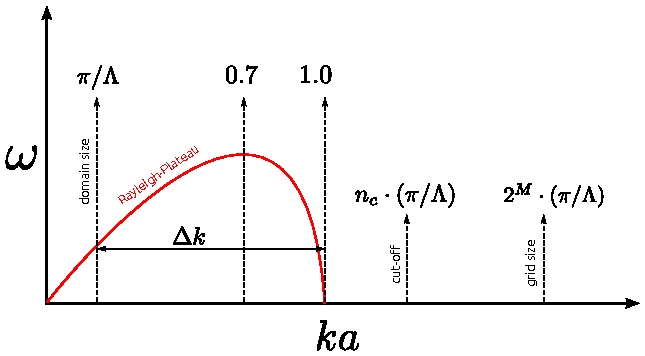
\includegraphics{plots/ligament_breakup/wave_quant.pdf}
\caption{ The dispersion relation of the Rayleigh-Plateau instability 
	\cite{rayleigh1879a, plateau1849}, expressing the growth rate of 
	the small amplitude perturbations as a function of 
	the reduced wavenumber \eqref{rayleigh_plateau}.
	The vertical dashed line A represents the upper limit
	to the perturbation wavelength, corresponding to the domain size $L$. 
	At the opposite end of the spectrum, E represents smallest wavelength  
        limited by the grid size $1/2^M$, where $M$ is the maximum level of 
	resolution for our octree grid. B corresponds to the wavenumber with 
	the maximum growth based on linear theory, whereas C represents the limit
	beyond which all perturbations are stable. The number of discrete modes
	that fall within the unstable part of the spectrum ($\Delta K$) 
	is a linear function of the ligament aspect ratio. 
	}
\label{quant}
\end{figure}

A similar analysis for the full Navier-Stokes equations 
was carried out by Chandrasekhar \cite{chandra}. 
The corresponding dispersion relation for viscous 
flows incorporating the long wavelength approximation 
of Weber \cite{weber1931}, at the limit of low Reynolds is given by

\begin{align}
\omega = \frac{\omega_\mu}{6}\left(1 - x^2 \right) , 
\label{weber_chandra}
\end{align}

where $\omega_\mu = \sigma / \mu a $. 
A similar conclusion can be drawn from \eqref{weber_chandra},
that all the perturbations correponding to $x \geq 1 $ are 
stable with respect to linear theory. 
\marginnote{
}
In Fig. \ref{quant}, we illustrate this principle using the dispersion 
relation of the inviscid Rayleigh-Plateau instability as a toy model. 
As one can observe, the number of discrete modes in the unstable part
of the spectrum amongst the $n_c$ modes initially excited is given by 

\begin{align}
 \Delta k = \Lambda / \pi - 1 .  
\end{align}

Thus, the aspect ratio ($\Lambda$) of our ligaments is the parameter 
responsible for selecting the number of modes actually playing a 
role in the destabilization of the ligament into the eventual drops. 
To this effect, in the present study we opt to study the dynamics of 
slender ligaments i.e. large aspect ratios, so that we excite a large enough 
number of discrete frequencies that are unstable with respect to linear theory. 
The expectation is that the competition and interactions \sidenote{
Beyond the exponential and independent growth phase of the 
modes in the linear regime, non-linear effects eventually 
kick into place, hence the interaction between the different modes.
}
between these unstable modes will play a key role in the
complex liquid rearrangements within the ligament bulk. 

\subsection*{Numerical Fine Tuning}
As we have discussed in the previous part (A) of the thesis,  
one has to pay particular attention to several aspects pertaining to 
the numerical stability of solvers when dealing with surface tension 
dominated flows involving significant contrasts in material properties 
across the interface (such as our system of water ligaments in air). 
In our case with `Basilisk', we opt to use the standard non-conservative
formulation of the Navier-Stokes equations, which does not maintain 
consistency between mass and momentum transport. 
But, in this case we are able to circumvent effects such as `artificial
atomization' mainly due to two reasons :

\begin{marginfigure}
\centering
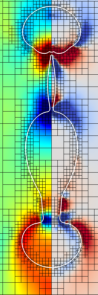
\includegraphics{plots/ligament_breakup/lig_mesh.pdf}
\caption{ Dynamically adapted octree meshes in the periphery 
of the interface location, with the refinement criteria based on
limiting gradients of volume fraction and velocity. The interface
is represented by the white contours, the colormap on the left half is
based on the axial velocity component, whereas the one on the right 
correponds to that of vorticity. 
The colors red and blue correspond to 
the higher and lower end values respectively, in case of both colormaps. 
	}
\label{lig_mesh}
\end{marginfigure}

\begin{itemize}
	\item The use of adaptive mesh refinement based on the octree grids in Basilisk allows 
		us to attain much higher levels of numerical resolution for the smaller/thinner 
		liquid structures, while using significantly coarser meshes away from the interface.
		For example, in our current simulations (see Fig. \ref{lig_mesh}), the number of cells
		in the domain (2D) are of the order $10^4$, whereas an equivalent \textit{uniform} mesh 
		(2D) would result in a problem size of order $10^6$, thereby differing by a factor of 100.
	\item The absence of the interaction of aerodynamic shear forces with the interface, in our particular
		problem configuration. This prohibits the `numerical mixing' of the gas velocity with the
		liquid density in the vicinity of poorly resolved interfacial cells, the concomitant 
		un-physical momentum tranfer resulting in the rapid destabilization of the interface.   
\end{itemize}

Furthermore, we have to tune the `knobs' of the 
solver concerning the criteria and corresponding 
thresholds regarding the dynamic mesh refinement. 
In all of the simulations/results demonstrated 
from this point onwards, the mesh adaptation is 
made according to the value of the local 
gradients of the volume fraction field, 
as well as local gradients of the velocity field components.  
The corresponding values of the thresholds are $10^{-3}$ 
and $10^{-1}$ for the volume fraction and velocity components respectively. 
The time step for the numerical integration is in itself dependent on the 
size of the smallest cells, as well as the local velocities. 
Therefore, we opt for a fixed CFL criteria in order to choose the time step, 
with the upper bound of the local CFL number throughout the domain being set to $0.05$.

\begin{marginfigure}[-6cm]
\centering
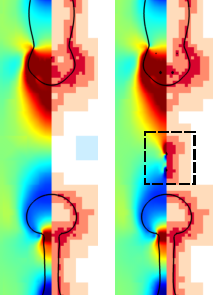
\includegraphics{plots/ligament_breakup/drop_removal.pdf}
	\caption{Illustration of the effects of our ``droplet removal'' feature, 
	with the figure on the left corresponding to simulations that filter out
	structures that are resolved by 10 cells or less, with the one on the right
	showing results with no droplet removal in place. The box (dashed line) in the 
	right hand side figure displays the extremely small structures that consume 
	a disproportionate amount of computational resources, without having any meaningful
	impact on the dynamics that we are interested in. 
	The colormap on the left side of the axis of 
	symmetry corresponds to the axial component of velocity, whereas the one on the right refers
	to the level of numerical resolution. The colors red and blue correspond to the higher 
	and lower end values respectively, in case of both colormaps. 
	}
\label{drop_remove}
\end{marginfigure}

Another numerical parameter that has a big influence on the performance of 
the numerical method is what we refer to as ``droplet removal'', 
which essentially removes extremely small and poorly 
resolved structures that float around in the domain. 
In our experience, these small `debris' like structures (see Fig. \ref{drop_remove})
hamper the simulations in several ways e.g. demanding extra computational 
resources in the form of additionally refined cells, 
or by imposing extremely small time steps (due to restrictions of 
local CFL number based on cell size) used for the numerical integration. 
The removal of these structures do not have any effect on the 
underlying dynamics of the breakups and coalescences, and their sizes 
are verified to be orders of magnitude below those corresponding to satellite drops. 
Our threshold for removal correponds to structures that are resolved by 10 cells or less. 
With regards to the iterative Poisson solver, we set a tolerance of $10^{-3}$, which in our
operator-split framework (see \eqref{ufinal}) corresponds to the 
accuracy by which the incompressibility condition \eqref{div} is verified. 

\subsubsection*{2D versus 3D}

An important question to ask ourselves before we conduct any large scale
study is the feasibility of carrying out full 3D simulations. 
In Basilisk, we have the option of carrying out axisymmetric simulations
that resolve the underlying governing equations on cylindrical coordinates. 
Due to the axial symmetry in the construction of our ligaments, carrying 
out 2D axisymmetric simulations instead of full 3D ones seem to offer a more 
computationally efficient approach, especially as we are interested in studying
the dynamics of thousands of such ligaments. 
We start with ligaments that correspond to the following parameters

\begin{align}
	Oh &= 10^{-2} \quad, \quad \varepsilon = 0.8 \quad , \\
	\Lambda &= 50 \quad , \quad K = 2\pi \quad .
\label{base_params}
\end{align}

The numerical resolution in our feasibility studies (in both 2D and 3D) correspond to 
$W / \Delta x_{\textrm{min}} = 10.24$, where $\Delta x_{\textrm{min}}$ is the size 
of the smallest grid cell in the octree (quadtree in 2D) mesh. 
The computations were carried out on 16 processors in parallel, within the framework
of parallelization through domain decomposition.
The computational times required to resolve the dynamics up to $T = 30$ are $54$ seconds 
and $976$ seconds for the 2D and 3D cases, respectively. 
In figures \ref{2d_3d_short} and \ref{2d_3d_long}, we illustrate the differences 
in the temporal evolution between a full 3D simulation and its 2D (axisymmetric)
equivalent, on fast and slow time scales respectively. 
As one can observe, the major qualitative difference 
lies in the excitation of certain azimuthal modes in the 3D case, 
which cannot be captured in the 2D case due to the 
imposition of symmetry about the central axis.
Such a subtle difference in the dynamics may 
explain the slightly higher tendency towards coalescence 
in the 2D case, due to the fact that some of the energy from 
the axial modes is transferred into the azimuthal modes in the 3D case. 
Apart from that, the 3D simulations also resolve some 
finer thread like structures that appear in the vicinity 
of the breakup region, the details of which are missing in the 2D simulations.  
Overlooking some finer aspects captured by the 3D simulations,  
there seem to be no major discrenible differences between the 2D and 3D simulations,
with the 2D simulations acting as an accurate reduced order model concerning the 
breakup and coalescence dynamics over both short and long time scales.
Looking at the feasibility in terms of computational resources, the 3D simulations 
are substantially more expensive than their 2D counterparts, by almost a factor of $20$ in most cases. 
Considering the fact that we plan to carry out thousands of such simulations, the 
slightly more accurate dynamics modeled by the 3D simulations do not justify the
approximately 20 fold increase in computational cost.   
Hence, from this point onwards unless mentioned otherwise, all of the 
simulations or results we present correspond to the 2D axisymmetric framework.

% Oh = 0.01 
% amp = 0.4
% K_cut = 50
% l/R = 100 (aspect ratio = 50)
% maxlevel = 9 

% 2D : 54 secs @ 16 procs 
% 3D : 976 secs @ 16 procs

\begin{figure*}
\centering
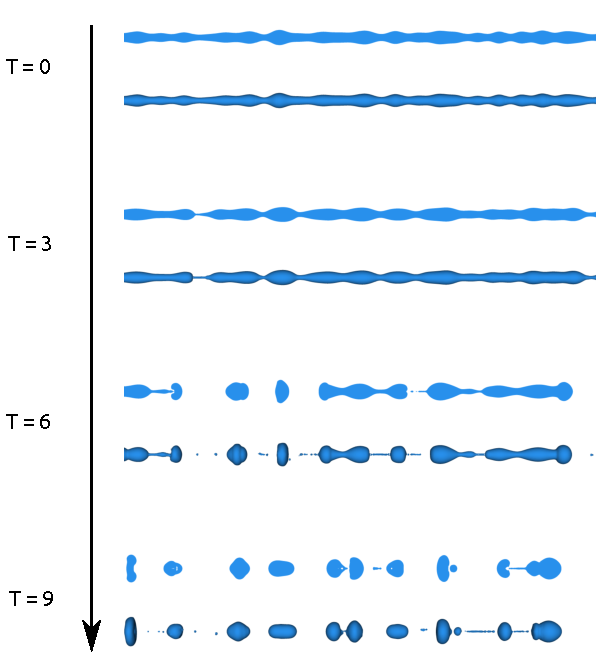
\includegraphics{plots/ligament_breakup/3d_vs_2d_short.pdf}
	\caption{Dynamics of the ligament destabilization, subsequent breakup 
	and eventual coalescences over \textit{short} time scales. 
	The physical parameters correspond to those defined in \eqref{base_params}.
	The top row (light blue) represents the geometrical reconstructions of 
	the interface shape for the 2D axisymmetric simulations, and the bottom 
	row (deep blue) represents those corresponding to the full 3D simulations.
	The discrepancy between the 3D and 2D cases in terms of distances between
	the neighbouring structures is merely an effect of the distortion of lengths
	in the 3D case, due to the use of a single point perspective (non-parallel) 
	projection in order to visualize the interface shapes. 
	}
\label{2d_3d_short}
\end{figure*}

\begin{figure*}
\centering
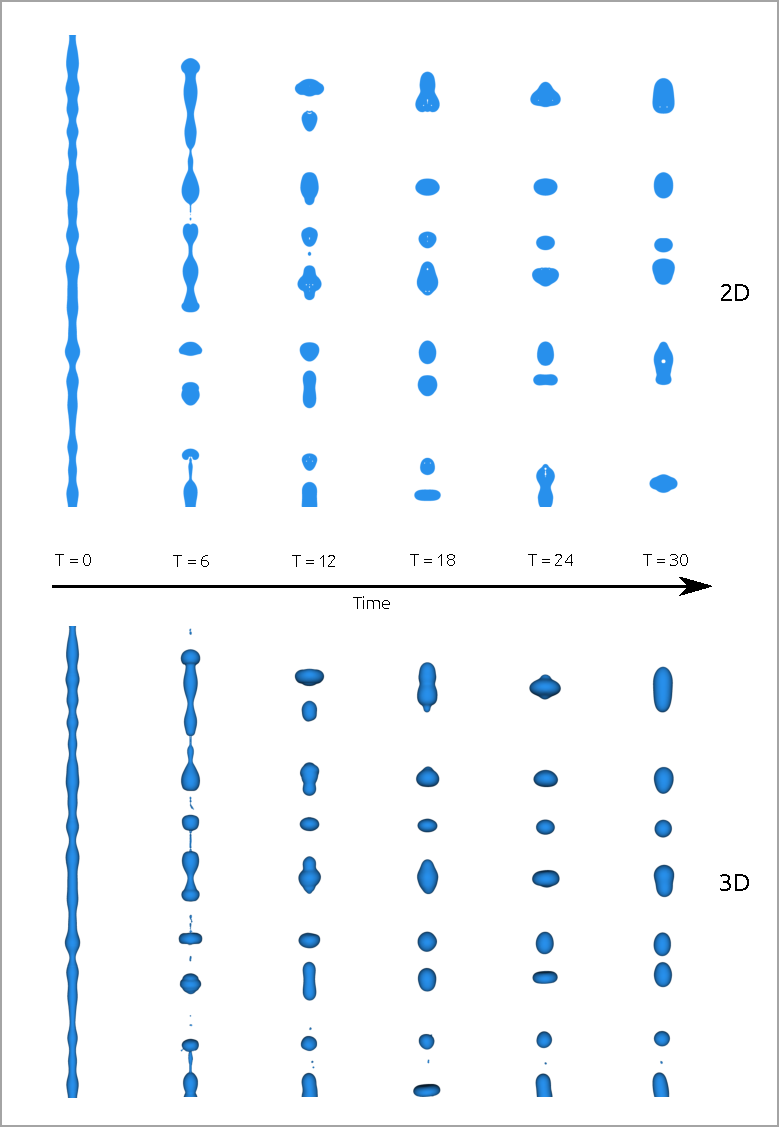
\includegraphics{plots/ligament_breakup/3d_vs_2d_long.pdf}
	\caption{Dynamics of the ligament destabilization, subsequent breakup 
	and eventual coalescences over \textit{long} time scales. 
	The physical parameters correspond to those defined in \eqref{base_params}.
	The top row (light blue) represents the geometrical reconstructions of 
	the interface shape for the 2D axisymmetric simulations, and the bottom 
	row (deep blue) represents those corresponding to the full 3D simulations.
	The discrepancy between the 3D and 2D cases in terms of distances between
	the neighbouring structures is merely an effect of the distortion of lengths
	in the 3D case, due to the use of a single point perspective (non-parallel) 
	projection in order to visualize the interface shapes. 
	}
\label{2d_3d_long}
\end{figure*}


\subsubsection*{Spatial Resolution}

Arguably the most important parameter on which the fidelity of our
numerical simulations hinges on is the spatial resolution or grid size. 
The octree structure in our solver entails successive refinements in the  
size of the cubic cell (square cell in 2D) by factors of $2$ in each direction.
\marginnote{In our simulations, the square domain of size $L$ has a minimum 
level of refinement corresponding to a grid size of $L/\Delta x = 2^{-4}$,
where $\Delta x$ is the size of the square cell.}  
As we have discussed before, we use the adaptive mesh refinement capabilities 
of Basilisk to add greater resolution to regions in the vicinity of the interface, 
therefore we have to impose an upper limit to the level of refinement as well. 
Henceforth, we refer to this upper limit as ``maxlevel'', 
where a ``maxlevel'' of $10$ correponds to a grid size of $L/ \Delta x = 2^{-10}$,  
In Fig. \ref{res_comp} we illustrate the differences between simulations carried out
using three different ``maxlevels'', corresponding to identical ligaments that
are characterized by the non-dimensional parameters given in \eqref{base_params}.
The computational cost of the most resolved simulation characterized by a ``maxlevel''
of $11$ ($W / \Delta x_{\textrm{min}} = 40.96$) is $516$ seconds\sidenote{
These simulations are carried out in parallel on 16 processors. }, 
for ``maxlevel'' of 10 ($W / \Delta x_{\textrm{min}} = 20.48$) is $156$ seconds, and finally 
for ``maxlevel'' of 9 ($W / \Delta x_{\textrm{min}} = 10.24$) is $54$ seconds. 
Comparing the simulations at the different resolutions, we do not observe any substantial 
differences in the dynamics at intermediate as well as long time scales.
\marginnote{
As a minor remark, we point out that coalescences take place marginally faster for the 
lower resolutions compared to the one as the ``maxlevel'' of $11$. 
}
Judging by the qualitative and quantitative similarities between the simulations corresponding 
to ``maxlevels'' $10$ and $11$, we conclude that our simulations are converged (more or less),
and that a ``maxlevel'' of $10$ serves as an optimal level of refinement for our future simulations.  

% same parameters, with l9,l10,l11 

% L11 : 516 secs @ 16 procs
% L10 : 156 secs @ 16 procs 
% L9  : 54 secs @ 16 procs 
\begin{figure*}
\centering
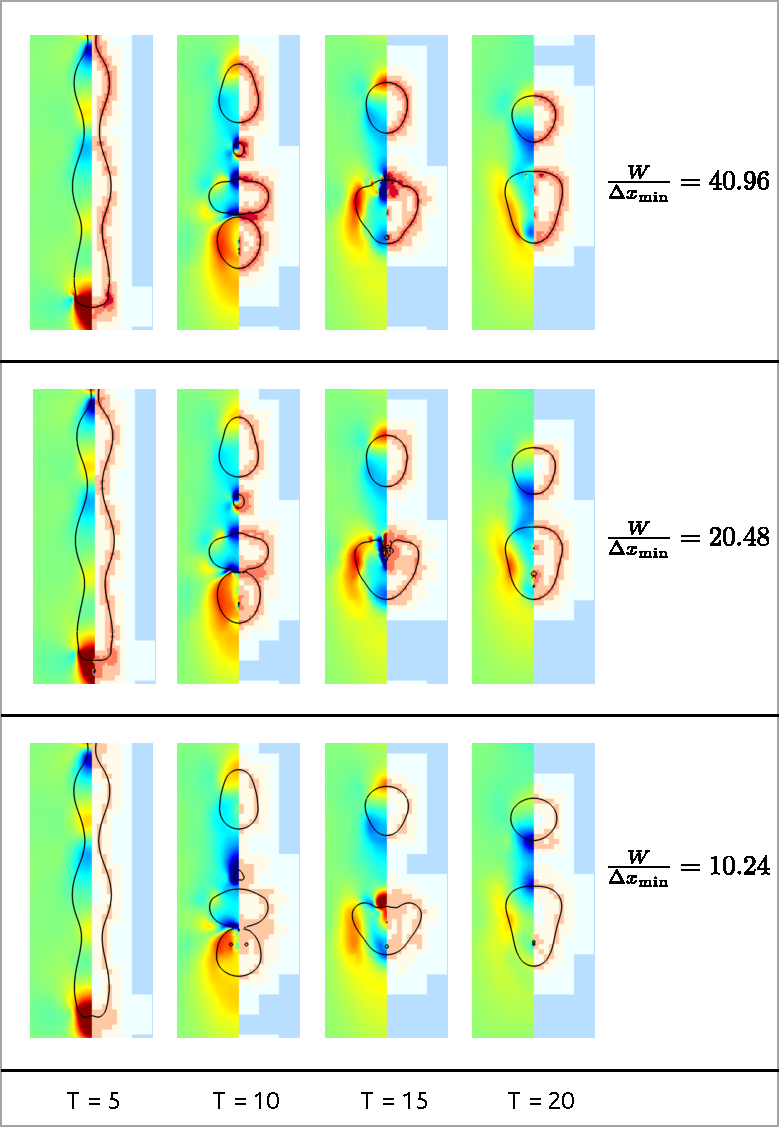
\includegraphics{plots/ligament_breakup/resolution_compare.pdf}
	\caption{Dynamics of the ligament destabilization (closeup), subsequent breakup 
	and eventual coalescences over \textit{intermediate} time scales.
	The top row represents simulations carried out at a ``maxlevel'' of $11$,
	the middle and bottom rows represents those carried out at ``maxlevels'' of
	$10$ and $9$ respectively. 
	The colormap is kept the same across all figures, where the left 
	side of the axis of symmetry in each figure corresponds to the axial component of 
	velocity (values from $-1$ to $1$), whereas the one on the right refers to 
	the \textit{level} of numerical resolution (from levels $4$ to $11$). 
	The colors red and blue correspond to the higher and lower 
	end values respectively, in case of both colormaps. 
	As one goes from the middle to the top row, there are no significant distinctions 
	between the interface shapes (black curves), especially at long time scales such as $T=20$. 
	}
\label{res_comp}
\end{figure*}



\section{Impact of Initial Conditions}

The characteristic length scale of the problem is the radius $R$ of our ligaments, 
which are in turn determined by the choice of Ohnesorge number, given that we are dealing with air-water systems.
On the other hand, the global dynamics of the ligament breakup take place over a multitude of different time scales, 
in particular the penultimate stages of the non-linear breakup which occur on successively shrinking (faster) time scales.  
We direct our attention towards understanding the dynamics over much larger time scales rather than those  
associated with the self-similar collapse of the liquid bridges that lead to the formation of drops. 
In this study, we loosely define \textit{short} time scales as intervals $\Delta t$ corresponding 
to $ \Delta t \leq 2T $, \textit{intermediate} ones as $ 2 < \Delta t \leq 4T $ 
and \textit{long} time scales as intervals $\Delta t \geq 5T$. 
The combination of $Oh$, $\varepsilon$, $\Lambda$ and $K$ used to 
characterize our problem also act as initial conditions that specify the 
randomly corrugated geometrical shape of the ligament.  
In this section, we take a closer look at the differences in the dynamics of ligament destabilization 
and the ensuing coalescences brought about by the difference in the initial shapes of the ligament in question.

\paragraph{Corrugation Amplitude}
The parameter $\varepsilon$ acts as a quantitative measure of the ``smoothness'' 
of the initial surface profile, being defined as the standard deviation of the 
un-filtered white noise signal rescaled by the mean radius of the ligament.



\paragraph{Ohnesorge Number}

\paragraph{Cut-Off Frequency}

\paragraph{Aspect-Ratio}




\begin{figure*}
\centering
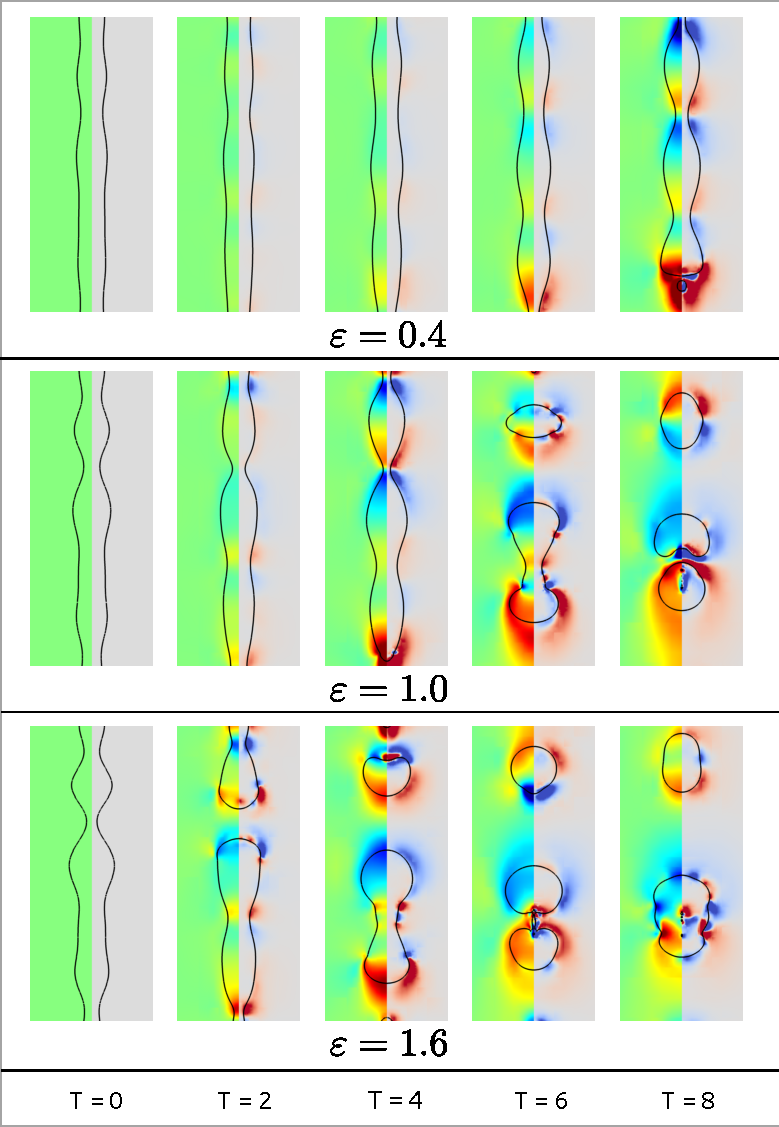
\includegraphics{plots/ligament_breakup/amplitude_compare.pdf}
	\caption{Dynamics of the ligament destabilization (closeup), subsequent breakup 
	and eventual coalescences over \textit{short} time scales.
	Simulations of identical ligament surface profiles
	subject to different initial corrugation amplitudes, with the smallest 
	amplitude represented by the top row and the largest amplitude by the bottom row. 
	The colormap is kept the same across all figures, where the left 
	side of the axis of symmetry in each figure corresponds to the axial component of 
	velocity (values from $-1$ to $1$), whereas the one on the right refers to 
	the vorticity (values from $-1$ to $1$) perpendicular to the plane. 
	The colors red and blue correspond to the higher and lower 
	end values respectively, in case of both colormaps. 
	The interface shapes are represented by the black contours.
	}
\label{amp_comp}
\end{figure*}


\begin{figure*}
\centering
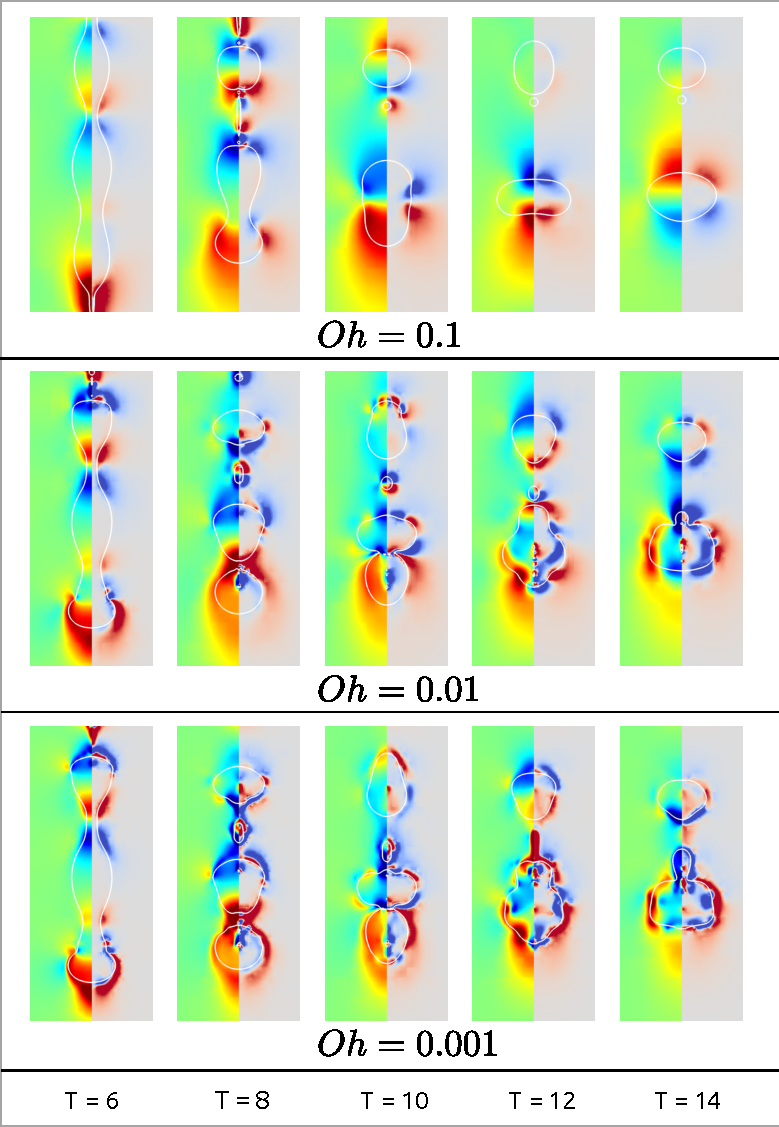
\includegraphics{plots/ligament_breakup/ohnesorge_compare.pdf}
	\caption{Dynamics of the ligament destabilization (closeup), subsequent breakup 
	and eventual coalescences over \textit{intermediate} time scales.
	Simulations of identical ligament surface profiles
	at different length scales in accordance with the  
	Ohnesorge numbers that characterize them, with the smallest 
	length scale represented by the top row ($Oh = 0.1$) and the largest 
	length scale by the bottom row ($Oh = 0.001$). 
	The colormap is kept the same across all figures, where the left 
	side of the axis of symmetry in each figure corresponds to the axial component of 
	velocity (values from $-1$ to $1$), whereas the one on the right refers to 
	the vorticity (values from $-1$ to $1$) perpendicular to the plane. 
	The colors red and blue correspond to the higher and lower 
	end values respectively, in case of both colormaps. 
	The interface shapes are represented by the white contours.
	}
\label{ohne_comp}
\end{figure*}


\begin{figure*}
\centering
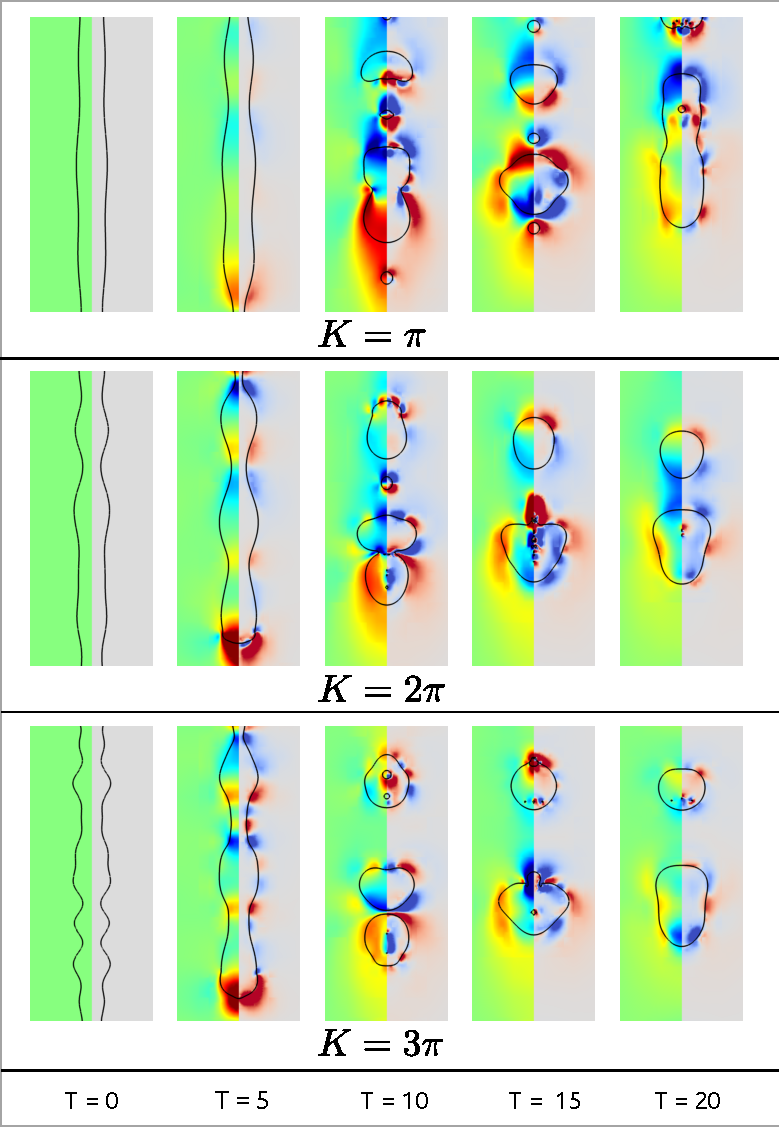
\includegraphics{plots/ligament_breakup/wave_compare.pdf}
	\caption{Dynamics of the ligament destabilization (closeup), subsequent breakup 
	and eventual coalescences over \textit{intermediate} time scales.
	Simulations of ligament surface profiles that differ due to the 
	different set of random waves used to generate them, with the 
	profile corresponding to the lowest cut-off frequency represented 
	by the top row and the highest cut-off by the bottom row. 
	The colormap is kept the same across all figures, where the left 
	side of the axis of symmetry in each figure corresponds to the axial component of 
	velocity (values from $-1$ to $1$), whereas the one on the right refers to 
	the vorticity (values from $-1$ to $1$) perpendicular to the plane. 
	The colors red and blue correspond to the higher and lower 
	end values respectively, in case of both colormaps. 
	The interface shapes are represented by the black contours.
	}
\label{wave_comp}
\end{figure*}


\begin{figure*}
\centering
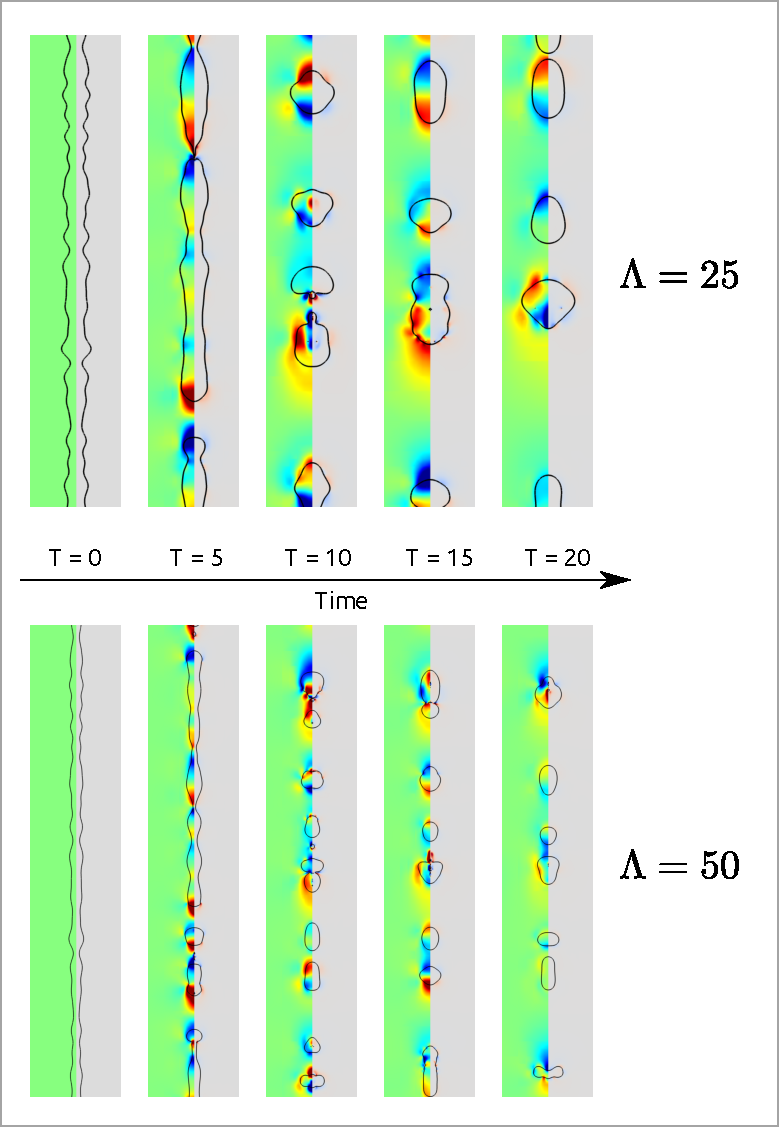
\includegraphics{plots/ligament_breakup/aspect_compare.pdf}
	\caption{Dynamics of the ligament destabilization, subsequent breakup 
	and eventual coalescences over \textit{intermediate} time scales.
	Simulations for identical ligament surface profiles
	corresponding to different aspect ratios (having identical radii), 
	with the shorter ligament represented by the top row and the longer one by the bottom row. 
	The colormap is kept the same across all figures, where the left 
	side of the axis of symmetry in each figure corresponds to the axial component of 
	velocity (values from $-1$ to $1$), whereas the one on the right refers to 
	the vorticity (values from $-1$ to $1$) perpendicular to the plane. 
	The colors red and blue correspond to the higher and lower 
	end values respectively, in case of both colormaps. 
	The interface shapes are represented by the black contours.
	}
\label{asp_comp}
\end{figure*}

